% Options for packages loaded elsewhere
% Options for packages loaded elsewhere
\PassOptionsToPackage{unicode}{hyperref}
\PassOptionsToPackage{hyphens}{url}
\PassOptionsToPackage{dvipsnames,svgnames,x11names}{xcolor}
%
\documentclass[
]{article}
\usepackage{xcolor}
\usepackage[margin=1in]{geometry}
\usepackage{amsmath,amssymb}
\setcounter{secnumdepth}{-\maxdimen} % remove section numbering
\usepackage{iftex}
\ifPDFTeX
  \usepackage[T1]{fontenc}
  \usepackage[utf8]{inputenc}
  \usepackage{textcomp} % provide euro and other symbols
\else % if luatex or xetex
  \usepackage{unicode-math} % this also loads fontspec
  \defaultfontfeatures{Scale=MatchLowercase}
  \defaultfontfeatures[\rmfamily]{Ligatures=TeX,Scale=1}
\fi
\usepackage{lmodern}
\ifPDFTeX\else
  % xetex/luatex font selection
\fi
% Use upquote if available, for straight quotes in verbatim environments
\IfFileExists{upquote.sty}{\usepackage{upquote}}{}
\IfFileExists{microtype.sty}{% use microtype if available
  \usepackage[]{microtype}
  \UseMicrotypeSet[protrusion]{basicmath} % disable protrusion for tt fonts
}{}
\usepackage{setspace}
\makeatletter
\@ifundefined{KOMAClassName}{% if non-KOMA class
  \IfFileExists{parskip.sty}{%
    \usepackage{parskip}
  }{% else
    \setlength{\parindent}{0pt}
    \setlength{\parskip}{6pt plus 2pt minus 1pt}}
}{% if KOMA class
  \KOMAoptions{parskip=half}}
\makeatother
% Make \paragraph and \subparagraph free-standing
\makeatletter
\ifx\paragraph\undefined\else
  \let\oldparagraph\paragraph
  \renewcommand{\paragraph}{
    \@ifstar
      \xxxParagraphStar
      \xxxParagraphNoStar
  }
  \newcommand{\xxxParagraphStar}[1]{\oldparagraph*{#1}\mbox{}}
  \newcommand{\xxxParagraphNoStar}[1]{\oldparagraph{#1}\mbox{}}
\fi
\ifx\subparagraph\undefined\else
  \let\oldsubparagraph\subparagraph
  \renewcommand{\subparagraph}{
    \@ifstar
      \xxxSubParagraphStar
      \xxxSubParagraphNoStar
  }
  \newcommand{\xxxSubParagraphStar}[1]{\oldsubparagraph*{#1}\mbox{}}
  \newcommand{\xxxSubParagraphNoStar}[1]{\oldsubparagraph{#1}\mbox{}}
\fi
\makeatother


\usepackage{longtable,booktabs,array}
\newcounter{none} % for unnumbered tables
\usepackage{calc} % for calculating minipage widths
% Correct order of tables after \paragraph or \subparagraph
\usepackage{etoolbox}
\makeatletter
\patchcmd\longtable{\par}{\if@noskipsec\mbox{}\fi\par}{}{}
\makeatother
% Allow footnotes in longtable head/foot
\IfFileExists{footnotehyper.sty}{\usepackage{footnotehyper}}{\usepackage{footnote}}
\makesavenoteenv{longtable}
\usepackage{graphicx}
\makeatletter
\newsavebox\pandoc@box
\newcommand*\pandocbounded[1]{% scales image to fit in text height/width
  \sbox\pandoc@box{#1}%
  \Gscale@div\@tempa{\textheight}{\dimexpr\ht\pandoc@box+\dp\pandoc@box\relax}%
  \Gscale@div\@tempb{\linewidth}{\wd\pandoc@box}%
  \ifdim\@tempb\p@<\@tempa\p@\let\@tempa\@tempb\fi% select the smaller of both
  \ifdim\@tempa\p@<\p@\scalebox{\@tempa}{\usebox\pandoc@box}%
  \else\usebox{\pandoc@box}%
  \fi%
}
% Set default figure placement to htbp
\def\fps@figure{htbp}
\makeatother





\setlength{\emergencystretch}{3em} % prevent overfull lines

\providecommand{\tightlist}{%
  \setlength{\itemsep}{0pt}\setlength{\parskip}{0pt}}



 


\makeatletter
\@ifpackageloaded{caption}{}{\usepackage{caption}}
\AtBeginDocument{%
\ifdefined\contentsname
  \renewcommand*\contentsname{Table of contents}
\else
  \newcommand\contentsname{Table of contents}
\fi
\ifdefined\listfigurename
  \renewcommand*\listfigurename{List of Figures}
\else
  \newcommand\listfigurename{List of Figures}
\fi
\ifdefined\listtablename
  \renewcommand*\listtablename{List of Tables}
\else
  \newcommand\listtablename{List of Tables}
\fi
\ifdefined\figurename
  \renewcommand*\figurename{Figure}
\else
  \newcommand\figurename{Figure}
\fi
\ifdefined\tablename
  \renewcommand*\tablename{Table}
\else
  \newcommand\tablename{Table}
\fi
}
\@ifpackageloaded{float}{}{\usepackage{float}}
\floatstyle{ruled}
\@ifundefined{c@chapter}{\newfloat{codelisting}{h}{lop}}{\newfloat{codelisting}{h}{lop}[chapter]}
\floatname{codelisting}{Listing}
\newcommand*\listoflistings{\listof{codelisting}{List of Listings}}
\makeatother
\makeatletter
\makeatother
\makeatletter
\@ifpackageloaded{caption}{}{\usepackage{caption}}
\@ifpackageloaded{subcaption}{}{\usepackage{subcaption}}
\makeatother
\usepackage{bookmark}
\IfFileExists{xurl.sty}{\usepackage{xurl}}{} % add URL line breaks if available
\urlstyle{same}
\hypersetup{
  pdftitle={SEPTA Metro and Trolley: A Guide for a New Penn Student},
  pdfauthor={Yixin Yang},
  colorlinks=true,
  linkcolor={blue},
  filecolor={Maroon},
  citecolor={Blue},
  urlcolor={Blue},
  pdfcreator={LaTeX via pandoc}}


\title{SEPTA Metro and Trolley: A Guide for a New Penn Student}
\author{Yixin Yang}
\date{Invalid Date}
\begin{document}
\maketitle


\setstretch{1.5}
\subsection{Introduction}\label{introduction}

For a new student at the University of Pennsylvania (Penn), public
transportation is an important part of getting around Philadelphia.
Students may need to travel to different neighborhoods, shopping areas,
restaurants, or other parts of the city. SEPTA provides several types of
public transportation, including Metro and trolley services. However,
for someone who is new to Philadelphia, it can be difficult to
understand which lines and stations are most convenient from the Penn
campus.

In this project, I used web scraping to collect SEPTA transportation
information and answer a practical question: \emph{Which SEPTA Metro and
Trolley lines are most accessible to a new Penn student?}

The data came from the OpenDataPhilly website, specifically the SEPTA
``Routes, Stops, and Locations'' dataset. I used the \texttt{rvest}
package in R to scrape the webpage and identify the available CSV data
files. I then used the station and stop datasets to examine SEPTA Metro
and trolley routes. The datasets contain information such as route
names, station or stop names, and geographic coordinates.

For the Metro data, I used the High Speed Stations dataset. It contains
information for three main routes in the dataset: B, L, and M. For the
trolley data, I used the Trolley Stations dataset, which contains
trolley stop names, route abbreviations, and latitude and longitude
coordinates.

After collecting the data, I cleaned the datasets and combined the Metro
and trolley information. I used an approximate location for the Penn
campus as the reference point. Then, I calculated the approximate
straight-line distance between Penn and each SEPTA station or trolley
stop. This allowed me to compare the geographic accessibility of
different SEPTA lines.

\subsection{Results}\label{results}

The first chart shows the nearest SEPTA Metro or trolley stop for each
route. The trolley stops around 36th Street and 33rd Street are very
close to Penn. The L Line also has a station at 34th Street, which is
approximately 0.27 miles from the reference point on the Penn campus.
These locations are particularly close compared with some other SEPTA
routes.

\begin{figure}

\centering{

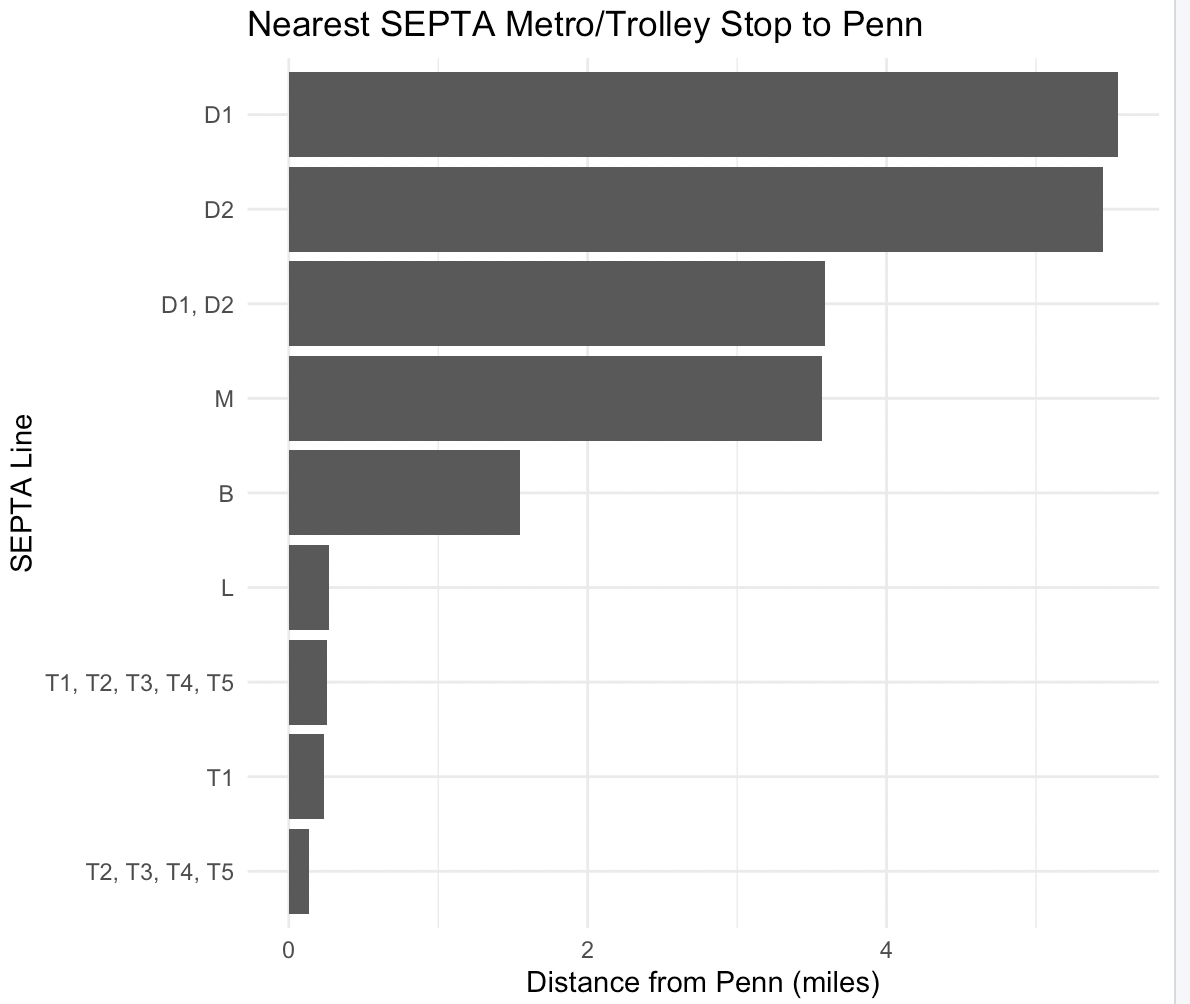
\includegraphics[width=0.85\linewidth,height=\textheight,keepaspectratio]{picture1.png}

}

\caption{\label{fig-chart1}Nearest SEPTA Metro or Trolley Stop to Penn}

\end{figure}%

The B Line has a nearby station at Walnut--Locust, although it is
farther from Penn than the L Line and the trolley stops. The M Line and
D routes have their closest stops several miles away from Penn.
Therefore, based only on geographic distance, these routes are less
directly accessible from the Penn campus.

The second chart shows the number of SEPTA stops within one mile of
Penn. The results show that several trolley routes and the L Line have
stops within this distance. This provides another way to understand
which routes may be convenient for a student who wants to walk to a
SEPTA stop.

\begin{figure}

\centering{

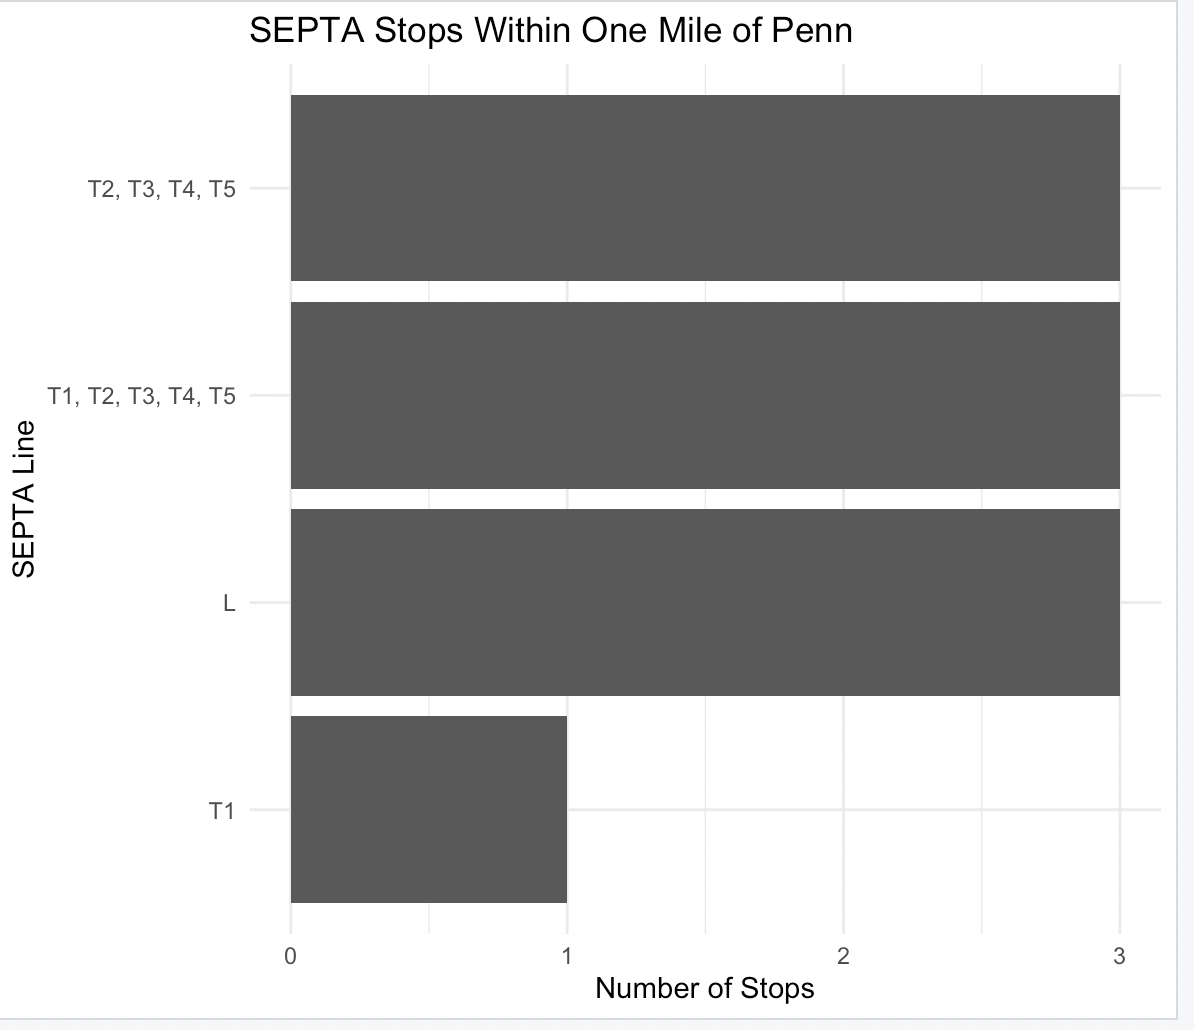
\includegraphics[width=0.85\linewidth,height=\textheight,keepaspectratio]{picture2.png}

}

\caption{\label{fig-chart2}SEPTA Stops Within One Mile of Penn}

\end{figure}%

The third chart provides another visualization of the SEPTA
transportation data collected for this project.

\begin{figure}

\centering{

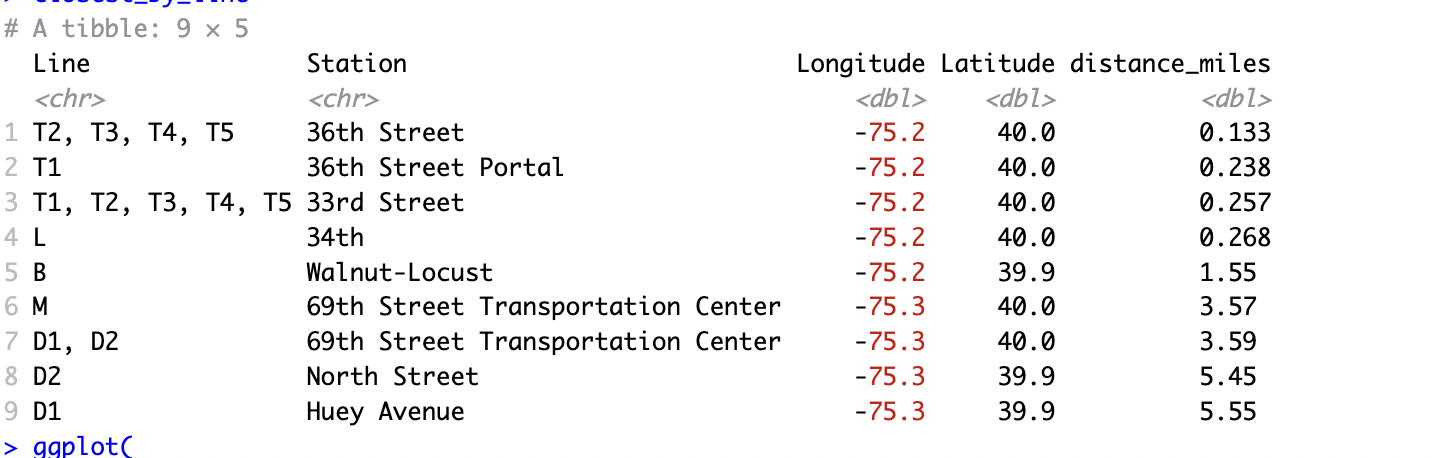
\includegraphics[width=0.85\linewidth,height=\textheight,keepaspectratio]{picture3.png}

}

\caption{\label{fig-chart3}SEPTA Metro and Trolley Data}

\end{figure}%

\subsection{Actionable Insight}\label{actionable-insight}

For a new Penn student, the results suggest that the trolley routes
around 33rd and 36th Streets and the L Line at 34th Street are
geographically close to campus. These routes may therefore be useful
starting points when learning how to use SEPTA.

The results also show why understanding the location of stops is useful.
A student does not necessarily need to know every SEPTA route
immediately. Instead, they can first learn the stations and trolley
stops that are closest to campus and then use those locations as
starting points for trips around Philadelphia.

However, distance alone does not determine whether a route is
convenient. Travel time, destination, service frequency, transfers, and
current service conditions can also affect the usefulness of a route.
Therefore, this analysis should be viewed as a simple geographic
comparison rather than a complete evaluation of SEPTA service.

\subsection{Limitations}\label{limitations}

There are several limitations to this analysis. First, the distance
calculation is an approximate straight-line distance rather than actual
walking distance. A station that is geographically close may require a
longer walking route because of streets, buildings, or other obstacles.

Second, some SEPTA stops are shared by multiple trolley routes. The
dataset may represent these routes together, so the route names in the
charts can sometimes appear as combinations such as T1, T2, T3, T4, and
T5.

Finally, the datasets used in this project are GIS datasets rather than
real-time service information. SEPTA schedules and service conditions
can change, so students should check current SEPTA information before
planning a specific trip.

\subsection{Conclusion}\label{conclusion}

This project demonstrates how web scraping can be used to answer a
practical transportation question. By scraping SEPTA information from
OpenDataPhilly and analyzing station locations in R, I was able to
compare the geographic accessibility of different Metro and trolley
routes from the Penn campus. The analysis shows that several trolley
stops and the L Line are located relatively close to Penn, providing
useful starting points for a new student learning to navigate
Philadelphia using SEPTA.




\end{document}
